\begin{figure}
    \centering
    \begin{subfigure}{.35\textwidth}
        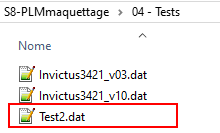
\includegraphics[width=.8\textwidth]{img/maj_file1.png}
        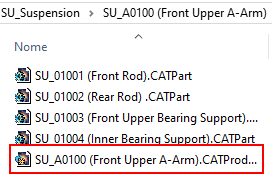
\includegraphics[width=\textwidth]{img/maj_file3.png}
    \end{subfigure}{}
    \begin{subfigure}{.3\textwidth}
        \centering
        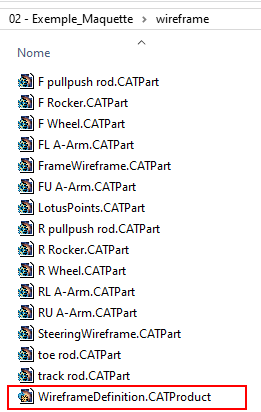
\includegraphics[width=\textwidth]{img/maj_file2.png}
    \end{subfigure}{}
    \begin{subfigure}{.3\textwidth}
        \centering
        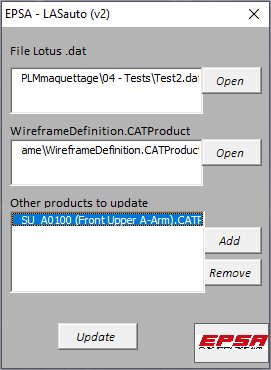
\includegraphics[width=\textwidth]{img/maj_screen.png}
    \end{subfigure}{}
    \caption{exemple de test de la macro}
    \label{fig:maj_assy}
\end{figure}